\documentclass[11pt,a4paper]{article}
\usepackage[margin=27mm]{geometry}
\usepackage[T1]{fontenc}
\usepackage{lmodern,microtype,amsmath,amssymb,amsthm,mathtools}
\usepackage{graphicx,booktabs,array,enumitem,listings,xcolor,fancyhdr}
\usepackage[numbers,sort&compress]{natbib}
\usepackage[colorlinks=true,allcolors=teal!65!black,breaklinks=true]{hyperref}
\usepackage{url}
\hypersetup{pdftitle={Local Exponential Gauges for Validated Contour Zero Counts},pdfauthor={Shivam Gupta},pdfsubject={Validated computational complex analysis}}
\setlength{\parskip}{4pt}
\setlength{\parindent}{1.2em}
\setlist{nosep,leftmargin=*}
\newtheorem{theorem}{Theorem}
\newtheorem{proposition}[theorem]{Proposition}
\newtheorem{corollary}[theorem]{Corollary}
\newtheorem{remark}[theorem]{Remark}
\DeclareMathOperator{\Arg}{Arg}
\DeclareMathOperator{\Impart}{Im}
\DeclareMathOperator{\Repart}{Re}
\newcommand{\CC}{\mathbb C}
\newcommand{\RR}{\mathbb R}
\newcommand{\cG}{\mathcal G}
\pagestyle{fancy}\fancyhf{}
\fancyhead[L]{\small Local exponential gauges for validated zero counts}
\fancyhead[R]{\small S. Gupta}\fancyfoot[C]{\thepage}
\setlength{\headheight}{14pt}
\lstset{basicstyle=\ttfamily\footnotesize,breaklines=true,frame=single,
 columns=fullflexible,backgroundcolor=\color{gray!3}}
\title{Local Exponential Gauges for\\Validated Contour Zero Counts}
\author{Shivam Gupta\\\small Independent Researcher, India\\
\small\href{mailto:shivam1720406@gmail.com}{shivam1720406@gmail.com}}
\date{17 October 2026}
\begin{document}
\maketitle
\begin{abstract}
Multiplying an analytic function by a nonvanishing exponential preserves its zeros but can greatly increase the work required by a disk-based contour certificate. We study this representation dependence for exponential polynomials with real exponents. On each straight contour panel, a local exponential factor is removed, a zero-excluding disk is verified, and the removed phase is restored analytically. The resulting certificates need neither a globally consistent choice of scale nor phase unwrapping of the original function values. We derive a convex scalar enclosure objective and a cancellation-preserving second-order variant with a logarithmic-derivative gauge. We prove soundness and common-exponent-shift invariance and give a replayable ball-arithmetic implementation. A deterministic study comprises 90 problems and 360 main certificates, followed by a 36-problem delay ablation, including logarithmic zero lattices, boundary-clearance tests, and single- and two-delay characteristic equations. Every count is checked at higher precision and against an independent reference. Comparisons include the best of nine fixed global gauges. The results identify a concrete tradeoff: local gauges can shorten certificates, while optimization and enclosure overhead can outweigh the savings. This is a method for reducing the cost of a specific class of validated certificates, rather than a universal acceleration of contour root finding.
\end{abstract}
\noindent\textbf{Keywords:} computational complex analysis; validated numerics; argument principle; exponential polynomials; delay equations.\\
\textbf{Software and reproducibility:} \url{https://github.com/shi1720/contourgauge}

\section{Introduction}
The argument principle converts an interior zero count into a boundary computation. In exact arithmetic, the count is unchanged when the characteristic function is multiplied by $e^{\kappa z}$. A certificate obtained by covering the image of the boundary with disks can behave differently: it must resolve the artificial growth and rotation introduced by this factor. This distinction matters when a characteristic equation admits several analytically equivalent normalizations, or when different exponential terms dominate on different parts of a contour.

Consider first $f(z)=e^{\kappa z}$. It has no zeros. A disk centered at the midpoint value on a panel of half-length $r$ obtained from the usual termwise exponential bound has relative radius $e^{|\kappa|r}-1$. A fixed safety threshold therefore forces $r=O(|\kappa|^{-1})$. Removing the known exponential leaves the constant function, which needs one disk per straight edge. This elementary example isolates representation cost without introducing a difficult zero problem. It does not imply that all argument-principle algorithms suffer this cost: logarithmic-derivative quadrature can handle a constant additive contribution very efficiently.

The more useful question is whether a local normalization can exploit changing term dominance without corrupting the accumulated winding. We answer this question for
\begin{equation}\label{eq:model}
 f(z)=\sum_{j=1}^J p_j(z)e^{\lambda_j z},\qquad \lambda_j\in\RR,
 \quad p_j\in\CC[z].
\end{equation}
The implemented inputs are rational exponents and rational real and imaginary polynomial coefficients. We use straight panels on a counterclockwise rectangle. The mathematical panel construction also applies to polygonal Jordan contours.

Our contributions are a panel certificate with an explicit phase correction; a convex, coefficient-weighted gauge-selection objective with a closed-form characterization between exponent knots; an invariance result that separates avoidable representation cost from genuine boundary difficulty; and an open implementation with replayable certificates and controlled numerical comparisons. The contribution is this particular enclosure, optimization, and replay workflow. The argument principle, nonvanishing exponential factors, interval arithmetic, and local logarithm branches are established tools.

\section{Related work and scope of the contribution}
Contour methods for analytic zero finding have a long history. Delves and Lyness \cite{delves1967} develop contour-based methods for locating zeros, and Kravanja and Van Barel \cite{kravanja2000} give a systematic treatment. Ying and Katz \cite{ying1988} study reliable argument-principle counting. The exponential convergence of analytic contour quadrature and its connection with root-finding moments are surveyed by Trefethen and Weideman \cite{trefethen2014}. We count zeros with multiplicity; we do not replace these methods for recovering their locations.

Certified sampled Nyquist tests already control the unobserved arcs between sampled values. Apkarian and Noll \cite{apkarian2018}, for example, derive a first-order variation test ensuring agreement between a true Nyquist arc and its polygonal replacement. Our test instead encloses an exponentially rescaled panel in a disk and records a continuous phase correction. We compare gauge policies within this test, rather than claiming that the underlying principle of certified sampling is new.

Exponential rescaling and analytic normalization are also well established in spectral computations. Evans-function algorithms preserve analyticity while controlling growth and decay; Barker et al. \cite{barker2018} discuss these issues together with Rouch\'e bounds and winding calculations. Their setting includes characteristic functions generated by differential equations. Here the input is an explicit exponential polynomial, and the normalization is chosen separately on each contour panel by an enclosure objective. The present experiments do not solve Evans-function boundary-value problems.

Validated integration supplies a natural independent reference. Petras \cite{petras2002} studies self-validating integration of piecewise analytic functions. Johansson \cite{johansson2017,johansson2018} develops efficient ball arithmetic and validated adaptive quadrature. We use Arb through python-flint for both the proposed verifier and an algorithmically independent integral of $f'/f$. These paths share an arithmetic library; they are not independent software stacks.

Delay characteristic equations are a classical application, including the scalar equation analyzed by Hayes \cite{hayes1950}. Lessard and Mireles James \cite{lessard2020} obtain validated eigenvalue counts by a broader functional-analytic approach. DDE-BIFTOOL \cite{ddebiftool} supplies established bifurcation and stability tools. Chonev, Ouaknine, and Worrell \cite{chonev2023} address much deeper decision questions for real zeros of exponential polynomials. Our termination statement assumes nonvanishing on a supplied compact contour and does not decide the general real-zero problem.

\begin{table}[t]
\centering\small
\begin{tabular}{p{.28\linewidth}p{.29\linewidth}p{.33\linewidth}}
\toprule
Established ingredient & Role in prior methods & Object studied here\\\midrule
Argument principle & Boundary counts and root moments & A rescaled panel phase record\\
Exponential normalization & Growth control without moving zeros & Local selection by an explicit enclosure objective\\
Certified sampled curves & Control between contour samples & Zero-excluding disks after local normalization\\
Ball arithmetic & Enclosures including rounding error & Replay without trusting the optimizer\\
Delay spectral analysis & Stability-determining roots & Complete unstable counts on bounded scalar examples\\
\bottomrule
\end{tabular}
\caption{The contribution boundary. None of the listed mathematical ingredients is claimed as a new principle.}
\label{tab:scope}
\end{table}

\section{A panel certificate with a local exponential gauge}
Let a straight oriented panel run from $a$ to $b$, and write
\begin{equation}
 m=(a+b)/2,\quad d=(b-a)/2,\quad z(t)=m+dt,\quad -1\le t\le1.
\end{equation}
Choose a real reference exponent $\lambda_*$ and define the exactly translated coefficients
\begin{equation}\label{eq:coeff}
 C_{jk}=e^{(\lambda_j-\lambda_*)m}\frac{p_j^{(k)}(m)d^k}{k!},
 \qquad 0\le k\le\deg p_j.
\end{equation}
The reference factor is constant on this panel and has no effect on its phase increment. Numerically, taking $\lambda_*$ to maximize $\lambda_j\Repart m$ keeps midpoint exponential magnitudes at most one. This range reduction is used in every comparator.

For any complex gauge center $s$, let
\begin{equation}\label{eq:gauge}
 G_s(t)=e^{-\lambda_*m-sdt}f(m+dt)
       =\sum_j\sum_k C_{jk}t^k e^{(\lambda_j-s)dt},
 \qquad F=G_s(0)=\sum_j C_{j0}.
\end{equation}
Define $r=|d|$, $u_j=r|\lambda_j-s|$, and
\begin{equation}\label{eq:bound}
 B(s)=\sum_j |C_{j0}|(e^{u_j}-1)
       +\sum_j\sum_{k\ge1}|C_{jk}|e^{u_j}.
\end{equation}
All sums over polynomial indices are finite. Fix $0<\eta<1$; the implementation uses $\eta=4/5$.

\begin{theorem}[Sound local phase certificate]\label{thm:panel}
If $B(s)<\eta|F|$, then $f$ is nonzero on the panel and its continuous change of argument is
\begin{equation}\label{eq:phase}
 \Delta\arg f=2\Impart(sd)+
 \Impart\left[\log\frac{G_s(1)}F-\log\frac{G_s(-1)}F\right],
\end{equation}
where both logarithms are principal logarithms. The gauge $s$ may be selected independently on each panel.
\end{theorem}
\begin{proof}
For $|t|\le1$, $|e^{wt}-1|\le e^{|w|}-1$ and $|e^{wt}|\le e^{|w|}$. Separating the constant polynomial coefficient in \eqref{eq:gauge} gives $|G_s(t)-F|\le B(s)$. Thus $G_s(t)/F$ lies in the disk $|w-1|<\eta$, which is contained in the open right half-plane. The principal logarithm is a single analytic branch on that disk, so its imaginary endpoint difference is the continuous argument change of $G_s$. The factor $e^{sdt}$ contributes $2\Impart(sd)$, and the constant factor $e^{\lambda_*m}$ contributes zero. No factor vanishes. The equality is a panelwise statement and requires no agreement of gauge choices on adjacent panels.
\end{proof}

\begin{corollary}[Certified zero count]\label{cor:count}
Suppose the ordered panels form a positively oriented polygonal Jordan contour $\Gamma$, and every panel satisfies Theorem~\ref{thm:panel}. Then
\begin{equation}\label{eq:count}
 N(f;\operatorname{int}\Gamma)=\frac1{2\pi}\sum_{I\subset\Gamma}\Delta_I\arg f.
\end{equation}
If a computed interval enclosing the right side contains exactly one integer, that integer is the zero count with multiplicity.
\end{corollary}
\begin{proof}
Theorem~\ref{thm:panel} establishes nonvanishing on the complete contour and the true continuous argument increment on every piece. Summation and the argument principle give \eqref{eq:count}. Interval enclosure and uniqueness of the contained integer establish the final assertion.
\end{proof}

\begin{figure}[t]
\centering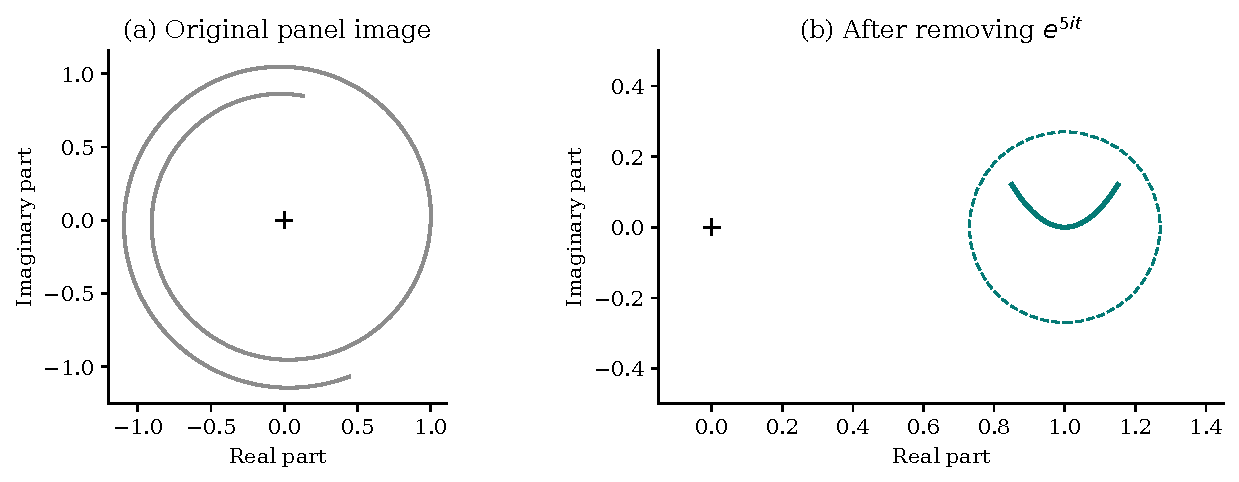
\includegraphics[width=\linewidth]{../figures/mechanism.pdf}
\caption{Illustrative panel geometry for $f(t)=e^{5it}(1+0.15t+0.12it^2)$. Removing the exponential leaves a curve in a disk of radius $0.27$ centered at one, so the logarithm has one branch. The removed phase increment is $10$ radians and is restored explicitly. This illustration is not a benchmark measurement.}
\label{fig:mechanism}
\end{figure}

\section{Choosing the gauge by a convex enclosure objective}
For real gauge centers, write
\begin{equation}
 A_j=|C_{j0}|,\qquad H_j=\sum_{k\ge1}|C_{jk}|,\qquad W_j=A_j+H_j.
\end{equation}
Then
\begin{equation}\label{eq:objective}
 B(s)=\sum_j W_j e^{r|\lambda_j-s|}-\sum_j A_j.
\end{equation}
The second term is constant in $s$. Unlike a center based only on the exponent range, this objective incorporates the local magnitudes of the translated polynomial coefficients.

\begin{proposition}[Existence and characterization of the optimal center]\label{prop:convex}
For a nondegenerate panel, if at least one $W_j>0$, the objective in \eqref{eq:objective} is strictly convex and coercive. Its unique minimizer belongs to the convex hull of the exponents with positive weight. Combine equal exponents and order the remaining ones as $\lambda_1<\cdots<\lambda_J$. On an open interval $(\lambda_k,\lambda_{k+1})$, put
\begin{equation}
 L_k=\sum_{j\le k}W_j e^{-r\lambda_j},\qquad
 R_k=\sum_{j>k}W_j e^{r\lambda_j}.
\end{equation}
An interior minimizer, when present, is
\begin{equation}\label{eq:closed}
 s_k=\frac{\log(R_k/L_k)}{2r}.
\end{equation}
Otherwise the minimizer is an exponent knot at which zero belongs to the subgradient.
\end{proposition}
\begin{proof}
For $r>0$, $s\mapsto e^{r|s-\lambda|}$ is strictly convex: it has positive second derivative away from its knot and an upward derivative jump at the knot. A positive weighted sum remains strictly convex and grows without bound as $|s|\to\infty$. To the left of every positive-weight exponent its derivative is negative, and to their right it is positive. Within the stated open interval, the objective up to its additive constant is $L_ke^{rs}+R_ke^{-rs}$. Setting its derivative to zero gives \eqref{eq:closed}. At a knot the usual subgradient criterion completes the characterization.
\end{proof}

Sorting, prefix sums, and suffix sums give a direct real-arithmetic search over knots and intervals. In a practical implementation, log-sum-exp avoids overflow. Our implementation instead uses a bounded scalar minimizer of the equivalent log-sum-exp objective, checks the knots and the midrange as additional candidates, and rounds the chosen offset to a dyadic rational with denominator $2^{30}$. This choice is intentionally outside the trusted verifier. The verifier recomputes \eqref{eq:bound} for the supplied rational center and accepts only a proved inequality. We make no claim that every numerical center attains the exact minimum.

\begin{proposition}[Small-panel limit]\label{prop:median}
For fixed $m$ and panel direction, as $r\downarrow0$, the gauge-dependent part of the first-order enclosure is
\begin{equation}\label{eq:median}
 \frac{B(s)}r\longrightarrow
 \sum_j |e^{(\lambda_j-\lambda_*)m}p_j(m)|\,|\lambda_j-s|
 +\sum_j |e^{(\lambda_j-\lambda_*)m}p'_j(m)|.
\end{equation}
Convergence is uniform for $s$ in a bounded interval. Consequently every accumulation point of exact optimal centers is a weighted median of the exponents, with weights $|e^{(\lambda_j-\lambda_*)m}p_j(m)|$, provided these weights are not all zero.
\end{proposition}
\begin{proof}
Use $e^{r|\lambda-s|}-1=r|\lambda-s|+O(r^2)$ uniformly on bounded sets. The $k=1$ coefficient has magnitude $r|e^{(\lambda_j-\lambda_*)m}p'_j(m)|$, and all higher ones are $O(r^2)$. Proposition~\ref{prop:convex} confines minimizers to a compact exponent interval. Uniform convergence then places their accumulation points in the minimizer set of the limiting weighted absolute-deviation objective, namely its weighted medians.
\end{proof}

This limit explains the adaptive behavior: where one term has more than half the midpoint weight, its exponent is the limiting center. It also identifies a limitation. Near strong cancellation, $|F|$ can be much smaller than the termwise coefficient magnitudes; an optimized bound can remain conservative.

\section{Preserving cancellation before enclosure}
\label{sec:jets}
The convex objective optimizes a bound that discards cancellation between terms. A second option retains the first two Taylor coefficients of the complete normalized function before taking absolute values. For $u_j=(\lambda_j-s)d$, define
\begin{equation}
 T_n=\sum_j\sum_{k=0}^{\min(n,\deg p_j)}
       C_{jk}\frac{u_j^{n-k}}{(n-k)!},\qquad n=0,1,2.
\end{equation}
For each term with $k\le2$, bound the remaining exponential series by
\begin{equation}
 R_{jk}=|C_{jk}|e^{|u_j|}\frac{|u_j|^{3-k}}{(3-k)!};
\end{equation}
for $k>2$, use $R_{jk}=|C_{jk}|e^{|u_j|}$. Let
\begin{equation}\label{eq:jetbound}
 B_2(s)=|T_1|+|T_2|+\sum_{j,k}R_{jk}.
\end{equation}

\begin{proposition}[A cancellation-preserving panel bound]\label{prop:jet}
For every complex $s$ and $|t|\le1$, $|G_s(t)-F|\le B_2(s)$. Either $B$ or $B_2$ may therefore be used in Theorem~\ref{thm:panel}. If $f(m)\ne0$, the exact choice $s=f'(m)/f(m)$ gives $T_1=0$. On compact sets separated from zeros, this exact logarithmic-derivative choice makes $B_2=O(r^2)$ as $r\to0$.
\end{proposition}
\begin{proof}
Expand every $t^k e^{u_jt}$ through total degree two. Its contribution to the polynomial part is included in $T_n$. For $k\le2$, the exponential Taylor remainder after degree $2-k$ is bounded by $e^{|u_j|}|u_j|^{3-k}/(3-k)!$ on $|t|\le1$. Terms with $k>2$ are bounded in full. The triangle inequality gives \eqref{eq:jetbound}. Direct differentiation of \eqref{eq:gauge} gives $T_1=d e^{-\lambda_*m}[f'(m)-sf(m)]$, so the stated choice cancels it. Bounded $s$, coefficients, and derivatives then give $T_2=O(r^2)$ and a remainder $O(r^3)$ uniformly.
\end{proof}

In floating-point search, the logarithmic derivative is only a proposal. We round its real and imaginary offsets to rational dyadic values and retain the verified, potentially nonzero $T_1$ in \eqref{eq:jetbound}. An exact $O(r^2)$ cancellation is not assumed for the rounded gauge. The implemented \emph{Jet} policy considers that proposal, the real convex proposal, the anchor, and zero, and selects the smallest computed enclosure. Its acceptance test uses the smaller of the two valid bounds. There is no convexity claim for $B_2$ and no claim that this candidate set optimizes it globally.

Taylor enclosures and logarithmic derivatives are classical. This variant tests a specific way to combine them with the local exponential phase record. To distinguish a better gauge from a better bound, the follow-up delay ablation gives the second-order enclosure to every comparator, including all nine fixed global centers.

\section{Invariance, representation cost, and termination}
\begin{theorem}[Common-exponent-shift invariance]\label{thm:shift}
Replace every $\lambda_j$ by $\lambda_j+\kappa$, with $\kappa\in\RR$, and every panel center $s$ by $s+\kappa$. Choose the reference exponent by the same term index. The coefficients $C_{jk}$, bounds $B$ and $B_2$, midpoint value $F$, and both normalized endpoint ratios in \eqref{eq:phase} are unchanged. The phase increment changes by $2\kappa\Impart d$. These changes sum to zero around a closed polygon.
\end{theorem}
\begin{proof}
The exponent differences in \eqref{eq:coeff} and \eqref{eq:gauge} are unchanged. The only remaining change in \eqref{eq:phase} is its explicit correction. Since $2d=b-a$ and the contour closes, the sum of corrections is $\kappa\Impart\sum(b-a)=0$.
\end{proof}

The exact optimizer is translation equivariant by uniqueness. The implementation optimizes offsets relative to the smallest exponent and quantizes those offsets, so its panel-selection computations also preserve common rational shifts. Final ball widths in the large phase correction can nevertheless grow with $|\kappa|$; the precision required to isolate the integer need not remain fixed.

\begin{proposition}[An avoidable linear certificate cost]\label{prop:cost}
For $f(z)=e^{\kappa z}$ on a polygon of perimeter $P$, using \eqref{eq:bound} with $s=0$ and threshold $\eta$ requires a number $n$ of panels satisfying
\begin{equation}
 n>\frac{P|\kappa|}{2\log(1+\eta)}.
\end{equation}
With $s=\kappa$, each original straight edge satisfies $B=0$ and needs one panel.
\end{proposition}
\begin{proof}
With $s=0$, the acceptance inequality is exactly $e^{|\kappa|r}-1<\eta$, hence every panel length $2r$ is smaller than $2\log(1+\eta)/|\kappa|$. Summing panel lengths gives the bound. With $s=\kappa$, $G_s$ is constant and nonzero.
\end{proof}

This comparison is between two disk certificates, not a complexity lower bound for zero counting itself. A global gauge already removes a common exponential perfectly. The purpose of local selection is to improve the remaining certificate where no single center tracks all dominant terms.

\begin{proposition}[Exact-arithmetic termination away from boundary zeros]\label{prop:terminate}
Suppose $f$ is nonzero on a compact polygonal contour. If gauge centers remain in a bounded interval, recursive bisection eventually gives $B(s)<\eta|F|$ on every panel.
\end{proposition}
\begin{proof}
On the compact contour, $|f|$ has a positive minimum. The finite set of possible reference exponents gives a positive lower bound on $|e^{-\lambda_*m}f(m)|$. Bounded centers, exponents, polynomial derivatives, and midpoint factors imply uniformly $B(s)=O(r)$ as $r\to0$. Thus sufficiently short panels pass.
\end{proof}
At finite precision the program may return unresolved because of rounding, a depth or work limit, or an actual boundary zero. It does not interpret failure to certify as evidence of a root. A precision-increase strategy can remove arithmetic limitations but cannot certify a contour that passes through a zero by this criterion.

\section{Implementation and certificate replay}
The reference implementation separates search from acceptance. A search record contains the exact rational model, the rectangle, and for every accepted panel its edge index, rational interval endpoints, and rational gauge center. It does not store a trusted count. Replay validates the rectangle orientation and the complete ordered partition, reconstructs translated coefficients, proves every disk inequality, encloses every phase increment, and isolates the final integer. A changed center or omitted panel must therefore pass the mathematics again.

All proof arithmetic uses python-flint 0.6.0 and Arb. The optimization uses NumPy 2.0.2 and SciPy 1.13.1. Rational strings are converted to balls by dividing exact integer numerator and denominator values. The midpoint exponent is removed before exponentiation, rather than evaluating a huge $f(m)$ and dividing afterward. The term $e^u-1$ is evaluated with \texttt{expm1} to avoid cancellation for small $u$. Optimizer weights may be ordinary floating-point approximations; they never decide acceptance.

\begin{lstlisting}[caption={Core search and verification contract (pseudocode).},label={alg:contract}]
for each oriented rectangle edge:
    stack = [(0, 1)]
    while stack is nonempty:
        interval = pop_leftmost(stack)
        center = propose_rational_gauge(model, interval)
        if ball_bound_B(center) < (4/5) * ball_abs_F:
            save(edge, interval, center)
        else:
            bisect interval, or return UNRESOLVED at the work limit
verify_geometry_and_partition(saved)
turns = sum(certified_phase(panel) for panel in saved) / (2*pi)
return unique_integer_in(turns), or UNRESOLVED
\end{lstlisting}

Replay is independent of the optimizer but currently shares the panel-enclosure code with search. This reduces the trusted code path but does not provide implementation diversity. Tests cover known multiple polynomial roots, nonzero exponentials, common-shift partition invariance, comparison of gauge objectives with a dense grid, rejection of corrupted certificates, and unresolved behavior at a boundary zero. The public verifier deliberately supports rectangles only; accepting a general polygon would require additional geometric validation.

\section{Experimental design}
\label{sec:experiments}
The deterministic suite uses seed 6402027 and contains 90 problems. Each is processed at 128 bits under four policies and replayed at 192 bits. The safety factor, bisection order, enclosure formula, and input representation are shared across policies. Search has maximum depth 28 and an attempt budget of 60,000. Inputs, counts, all panel records, timing samples, and environment information are archived in the repository.

\paragraph{Policies.}
\emph{None} uses $s=0$. \emph{Anchor} uses the first input exponent as a fixed global gauge. \emph{Midrange} uses the midpoint of the smallest and largest exponent. \emph{Local} uses the optimized panel proposal described above. All policies receive the same midpoint range reduction. In addition, an offline \emph{Fixed-9} comparator tests nine equally spaced global centers over the exponent range and retains the smallest complete certificate. It is an oracle over this finite grid, not a globally optimal fixed gauge. Its nine construction costs must not be interpreted as the cost of a single method.

\paragraph{Problems with explicit references.}
Five common-shift instances use
\begin{equation}
 e^{\kappa z}(e^z-1/2)(e^z-2)(e^z+1),
 \quad \kappa\in\{0,8,32,128,512\},
\end{equation}
on $[-2,2]+i[-7,7]$. They all have eight zeros. Nine dominance instances vary the contour width and exponent spacing for three-factor products. Four clearance instances use $(e^z-1)(e^z-2)$ on $[-\epsilon,2]+i[-5,5]$, with $\epsilon\in\{10^{-1},10^{-2},10^{-3},10^{-4}\}$. Another 36 instances use two to five randomly chosen nonzero rational real roots in the $w$-plane, expand $P(e^{\rho z})$ exactly, and vary $\rho\in\{1/2,1,2\}$ and a common exponent shift. Multiplicities are retained. Reference counts enumerate the explicitly known lattice
\begin{equation}\label{eq:lattice}
 z=\frac{\log w+2\pi i k}{\rho},\qquad P(w)=0,
\end{equation}
using ball logarithms and strict coordinate comparisons. The bounded frequency window makes the enumerated range $|k|\le100$ more than sufficient.

\paragraph{Delay equations.}
Twelve problems use $f(z)=z+1+be^{-\tau z}$, with $b\in\{1/2,2,4\}$ and $\tau\in\{1/2,1,2,4\}$, on $[0,3]+i[-20,20]$. Twenty-four seeded two-delay problems use
\begin{equation}\label{eq:multidelay}
 f(z)=z+1+b_1e^{-\tau_1z}+b_2e^{-\tau_2z},
\end{equation}
where $b_j$ are positive tenths in $[0.2,2.5]$, $\tau_1$ is in $[0.2,1.5]$, and $\tau_2$ is in $[1.6,4]$. Their rectangle is $[0,5]+i[-12,12]$. All 36 delay references independently integrate $f'/f$ around the rectangle by Arb adaptive quadrature at 192 bits, with absolute and relative tolerance goals $10^{-35}$. Acceptance requires a unique integer in the real part of $(2\pi i)^{-1}\int f'/f$ and an imaginary enclosure containing zero. Meromorphic ball evaluation supplies the required analytic-domain check for the integrator.

\paragraph{What is measured.}
Panel count measures certificate length; it is not the number of unique function evaluations. Construction time includes search and its first verification but excludes the subsequent 192-bit replay. Replay times are medians of five verifier calls at 192 bits. These are single-machine descriptive measurements with shared-library dependencies, rather than statistical estimates of a population of industrial models. The generated families are deliberately controlled; they are not a random sample of delay systems used in practice.

\section{Results}
All 360 main certificates were accepted and replayed successfully at 192 bits. Every count agrees with its reference. The 36 delay counts agree with independent validated quadrature; all 12 single-delay cases also agree with the analytic crossing calculation below. The nine test methods pass, including explicit corrupted-record rejection and an unresolved boundary-zero example.

On the common-shift family, the raw certificate grows from 102 panels at $\kappa=0$ to 29,344 at $\kappa=512$. The anchor policy uses 102 panels, the midrange policy 84, and the local policy 28 for every shift. Thus the local policy's improvement from removing the common factor must be distinguished from its additional improvement over a valid global normalization. Figure~\ref{fig:shift} makes this distinction explicit.

Outside the five shift instances, local gauges produce fewer panels than Fixed-9 on 66 of 85 problems, tie on 19, and produce more panels on none. The median paired Fixed-9/local panel ratios are 2.17 for dominance problems and 1.85 for the generated lattice family. Their family median panel counts are shown in Table~\ref{tab:panels}. This is evidence about the tested finite grid and sufficient bound, not a proof that local gauges outperform every fixed global center on every function.

The practical delay families show a much smaller benefit against a well-chosen fixed center: their median paired panel ratios are about 1.01 and 1.02. Comparing only with midrange would overstate the practical effect, because the zero or anchor center is already effective on many delay problems. The clearance family is also nearly tied with Fixed-9: as $\epsilon$ decreases from $10^{-1}$ to $10^{-4}$, local counts rise from 36 to 76 panels. Gauge optimization cannot remove a zero approaching the boundary.

Table~\ref{tab:times} and Figure~\ref{fig:paired} separate construction from replay. In the lattice family, the median midrange/local construction ratio is 0.73, so local construction is slower, while the corresponding replay ratio is 1.97. For the single-delay family the ratios are 0.67 and 2.14, but these timing gains in replay are relative to the less effective midrange policy. No general runtime superiority follows. In particular, certificate length is the more portable outcome: it does not depend on system load, while timings do.

\subsection{Follow-up: cancellation and a stronger fixed-gauge comparison}
The first study exposed small delay-family gains against Fixed-9. We therefore ran a follow-up ablation on all 36 delay problems, keeping the same contours, arithmetic precision, safety factor and reference counts. Each comparator may use the smaller of $B$ and $B_2$. The four policies are zero gauge, midrange, real local, and Jet; a fresh nine-center fixed sweep supplies a fifth comparison record. This follow-up is reported separately because it was motivated by the first study rather than specified before those results were inspected.

Every follow-up count agrees with its reference and replays at 192 bits. Jet gives fewer panels than the second-order Fixed-9 comparator on 26 problems and ties on ten, with no losses in this suite. The median paired Fixed-9/Jet panel ratios are 1.06 for the single-delay family and 1.07 for the two-delay family; the largest ratio is 1.28. This is a modest additional reduction, rather than an order-of-magnitude improvement. The real-local and Jet family medians are reported in Table~\ref{tab:cancel}; equal medians need not mean equal paired results.

The median fixed-certificate/Jet replay time ratios are 0.99 and 0.97. Thus the smaller Jet records do not produce a replay speedup on these examples: their more expensive enclosures outweigh the saved panels. This negative runtime result is part of the evidence. The second-order extension establishes an additional sound certificate and a small proof-length improvement on the tested delay models, while the simpler real-gauge certificate can remain the better computational choice.

\begin{table}[t]
\centering\small\begin{tabular}{lrrrrrr}\toprule
Family & $n$ & Fixed-9 & Real local & Jet & Panel ratio & Replay ratio\\\midrule
Delay & 12 & 42 & 41 & 39 & 1.06 & 0.99\\
Multidelay & 24 & 46 & 44 & 44 & 1.07 & 0.97\\
\bottomrule\end{tabular}
\caption{Follow-up delay ablation. All policies receive the cancellation-preserving enclosure. Panel columns are family medians; ratio columns are medians of paired Fixed-9/Jet ratios. A ratio above one favors Jet. Replay times are medians of five runs per record at 192 bits.}
\label{tab:cancel}
\end{table}
\begin{figure}[t]
\centering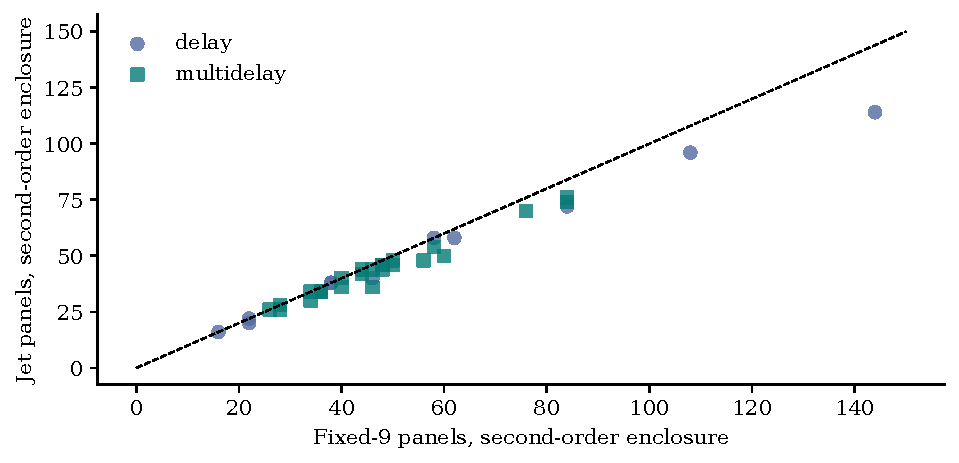
\includegraphics[width=.82\linewidth]{../figures/cancellation.pdf}
\caption{Second-order follow-up: Jet certificates versus the best of nine fixed real gauges, with the same two enclosure options supplied to both. The proof-length gain is small on many delay problems and does not translate into faster replay in the aggregate.}
\label{fig:cancel}
\end{figure}


\begin{figure}[t]
\centering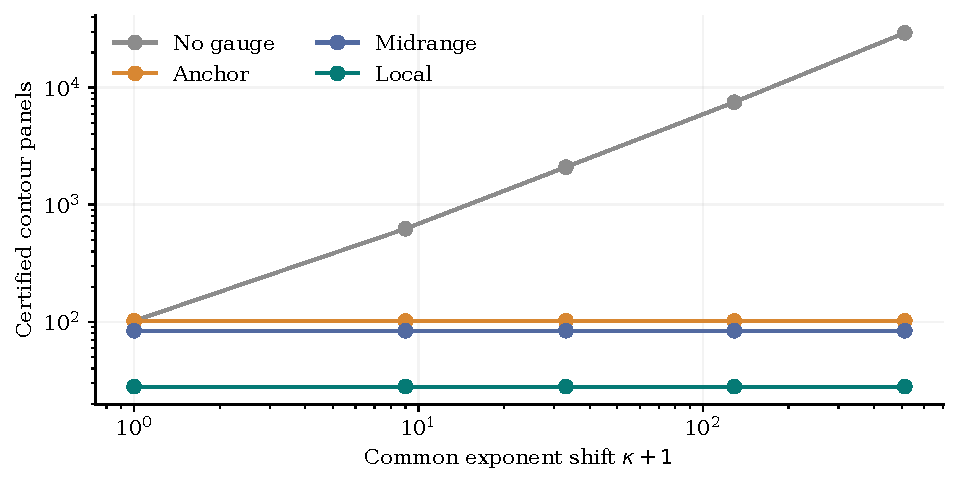
\includegraphics[width=.83\linewidth]{../figures/shift.pdf}
\caption{Representation stress test. The raw disk certificate grows with the common exponent shift. Every shifted problem has the same eight zeros. Anchor, midrange, and local gauges remove the common shift; local selection additionally exploits dominance around the contour. This experiment compares disk certificates and does not establish a weakness of logarithmic-derivative quadrature.}
\label{fig:shift}
\end{figure}

\begin{table}[t]
\centering\small\begin{tabular}{lrrrrrr}\toprule
Family & $n$ & None & Anchor & Midrange & Fixed-9 & Local\\\midrule
Dominance & 9 & 118 & 118 & 102 & 78 & 32\\
Clearance & 4 & 106 & 106 & 59 & 59 & 57\\
Lattice & 36 & 594 & 135 & 102 & 96 & 37.5\\
Delay & 12 & 47 & 47 & 109 & 47 & 45\\
Multidelay & 24 & 50 & 50 & 124 & 50 & 46\\
\bottomrule\end{tabular}
\caption{Median certificate panel counts. The five common-shift stress instances are excluded. Fixed-9 is the smallest certificate from nine tested fixed global centers for each problem. Medians are computed within a family; ratios of these medians are not paired effect estimates.}
\label{tab:panels}
\end{table}

\begin{table}[t]
\centering\small\begin{tabular}{lrrr}\toprule
Family & Fixed-9 / local panels & Construction ratio & Replay ratio\\\midrule
Dominance & 2.17 & 1.03 & 2.87\\
Clearance & 1.04 & 0.31 & 1.09\\
Lattice & 1.85 & 0.73 & 1.97\\
Delay & 1.01 & 0.67 & 2.14\\
Multidelay & 1.02 & 0.94 & 2.61\\
\bottomrule\end{tabular}
\caption{Median paired ratios. The first column compares Fixed-9 panel counts with local panel counts. Construction and replay ratios compare the midrange policy with local gauges. Values above one favor local gauges. Construction includes the first replay; separate replay measurements use 192 bits and five repetitions.}
\label{tab:times}
\end{table}

\begin{figure}[t]
\centering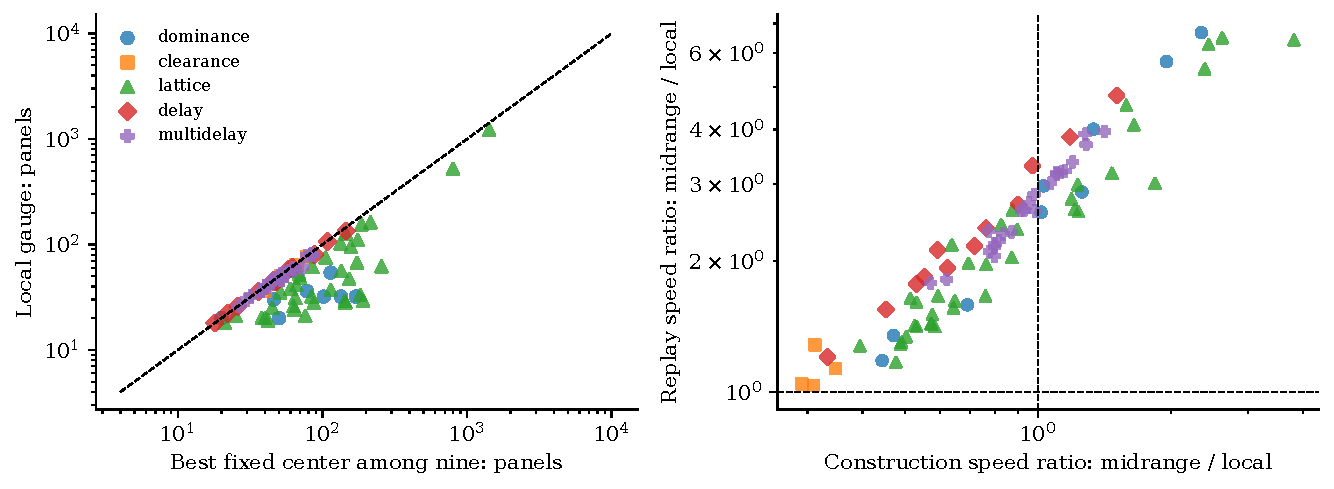
\includegraphics[width=\linewidth]{../figures/paired.pdf}
\caption{Paired comparisons outside the common-shift stress test. Left: local panel counts against the best tested fixed global center; below the diagonal indicates a shorter local certificate. Right: construction and replay speed ratios against the midrange policy. The upper-left quadrant represents the intended tradeoff: slower certificate construction but faster verification.}
\label{fig:paired}
\end{figure}

\section{Delay stability and practical interpretation}
For \eqref{eq:multidelay}, a root with $\Repart z\ge0$ must satisfy
\begin{equation}\label{eq:tail}
 |z+1|\le b_1+b_2.
\end{equation}
Since $b_1+b_2\le5$, no such root lies at $\Repart z\ge5$ or $|\Impart z|\ge12$. The chosen rectangle therefore contains every unstable root; successful certification on its left edge also excludes imaginary-axis roots. The same argument with a single coefficient $b\le4$ justifies the single-delay rectangle: at $\Repart z\ge3$ the exponential factor makes the right side strictly smaller than four, whereas $|z+1|\ge4$. Consequently the computed delay counts are full unstable-root counts, not just counts in an arbitrary spectral window.

For the single-delay cases a second analytic check is available. If $0<b<1$, \eqref{eq:tail} excludes any root in the closed right half-plane. If $b>1$, imaginary-axis crossings occur at
\begin{equation}\label{eq:crossing}
 \omega=\sqrt{b^2-1},\qquad
 \tau_k=\frac{\arccos(-1/b)+2\pi k}{\omega},\quad k=0,1,\ldots.
\end{equation}
At $z=i\omega$, implicit differentiation gives
\begin{equation}
 \frac1{z'(\tau)}=-\frac1{z(z+1)}-\frac\tau z,
 \qquad \Repart\frac1{z'(\tau)}=\frac1{b^2}>0.
\end{equation}
Thus each crossing pair moves from left to right. The unstable count starts at zero for small positive delay, by uniform convergence to $z+1+b$ on a compact half-disk containing all possible unstable roots. Away from crossing values it is twice the number of thresholds below $\tau$. This classical scalar analysis \cite{hayes1950} agrees with every single-delay certificate and quadrature reference. The two-delay cases do not use this formula.

\begin{figure}[t]
\centering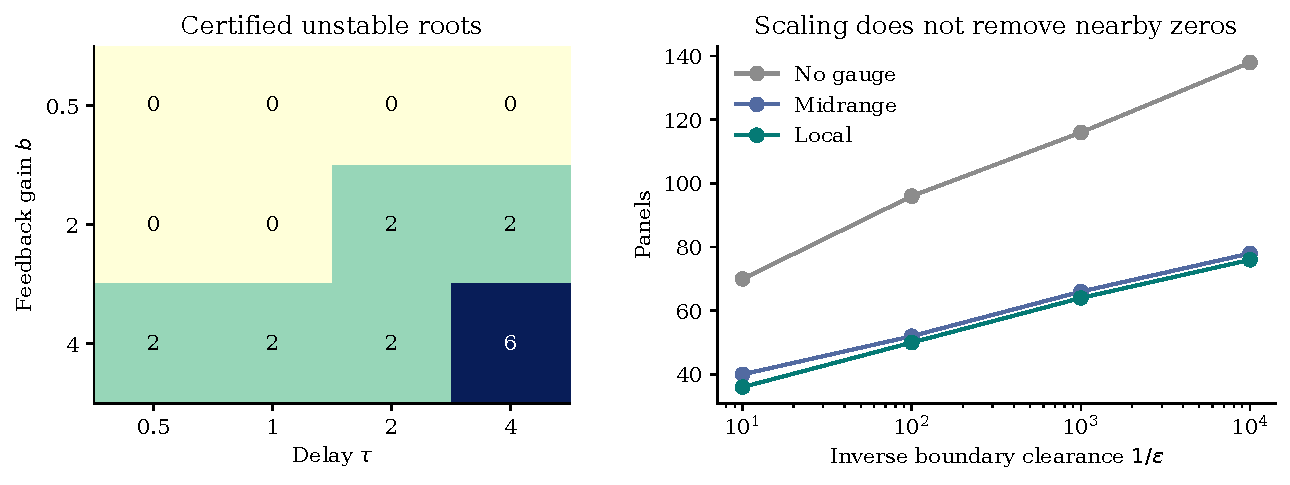
\includegraphics[width=\linewidth]{../figures/application.pdf}
\caption{Left: certified complete unstable counts for $z+1+be^{-\tau z}$; every cell also agrees with independent quadrature and the analytic crossing calculation. Right: certificate growth as a known zero approaches the contour. A local exponential gauge does not remove the need to resolve small boundary clearance.}
\label{fig:application}
\end{figure}

Delay stability is commercially relevant to process-control and feedback-design software. Existing systems already analyze delays directly or provide approximations, margins, and root corrections \cite{mathworks,ddebiftool}. The useful software object here is a compact, replayable spectral-count record attached to a model revision. A design tool could spend additional time constructing a short record and replay it during review or regression checking. The present study supports the numerical mechanism on explicit scalar models. It does not demonstrate customer demand, certification under a regulatory standard, or superiority over commercial control packages. A deployment would also need model provenance and uncertainty bounds; a certificate for an exact mathematical model cannot establish that the physical plant is modeled correctly.

\section{Limitations and further work}
The enclosure takes absolute values term by term. Severe cancellation, nearly vanishing boundary values, and high-degree polynomial factors can dominate the work. Common-shift invariance removes a representation artifact, not the conditioning of the zero problem. The exact convex optimizer minimizes one sufficient enclosure, not the total number of panels or wall-clock time. The implemented approximate optimizer may make a less favorable choice near a bisection threshold.

The empirical comparisons isolate gauge selection within a common verifier. The Fixed-9 sweep is a stronger fixed-gauge comparator than a single arbitrary center, but is not a continuous global optimization. We have not benchmarked against optimized implementations of Ying--Katz, DDE-BIFTOOL, or a complete suite of moment-based contour solvers. Independent quadrature is used to validate delay counts, not as a performance target. A generic claim of faster root counting would therefore be unsupported.

The current code treats real exponents, exact rational input data, explicit scalar functions, and rectangular contours; the Jet proposal may have a complex center. Complex input exponents would lead to a two-dimensional convex center problem and require a separate implementation and evaluation. Interval coefficients could encode model uncertainty; they would also require quantifying how the reference exponent, normalization, and endpoint logarithms vary across the family. Further reductions may come from higher-order panel models or merging neighboring records after search. These extensions are not part of the reported results.

\section{Conclusion}
Local exponential gauges turn a representation-dependent disk certificate into a panelwise normalization problem with explicit phase bookkeeping. The scalar enclosure objective is convex, has a concrete optimizer characterization, and approaches a weighted-median rule on short panels. Replay verifies the mathematics without trusting the gauge proposal. The experiments establish correct counts on the stated suite and show that proof length and construction speed are distinct design objectives. This makes local gauge selection a useful component for validated computational complex analysis, with a precisely bounded contribution and an auditable implementation.

\paragraph{Data and code availability.}
The repository contains the source, tests, exact inputs, every reported certificate, independent quadrature reference code, raw and summarized measurements, figure scripts, and this manuscript's \LaTeX\ source. The software is released under the MIT license. The paper and figures are released under CC BY 4.0. Reproduction commands and arithmetic dependencies are documented in the repository.

\bibliographystyle{plainnat}
\bibliography{references}

\appendix
\section{Reproduction and verification details}
From the repository root, create an isolated Python environment and install the project and plotting dependency. The following commands reproduce the test suite, main study, fixed-center sweep, and figures:
\begin{lstlisting}
python -m pip install -e . matplotlib==3.9.4
python -m unittest discover -s tests -v
python experiments/study.py
python experiments/global_sweep.py
python experiments/cancellation.py
python experiments/figures.py
python experiments/cancellation_figures.py
cd paper
tectonic main.tex
\end{lstlisting}
The archived measurements are observations of the recorded run; rerunning on another machine or under different load will change timings. Exact rational inputs, panel decisions away from thresholds, and certified counts should be stable. A finite-precision proof failure must be handled as unresolved, even when a reference count is available.

\section{Certificate format and trust boundary}
A certificate records the format, arithmetic precision, exact rational model and rectangle, and an ordered panel list. Each panel stores its edge, rational interval endpoints, and rational real or complex gauge. An optional enclosure-order field selects the second-order variant. The verifier checks exact rectangle orientation and complete interval coverage without gaps, overlaps or reversals. It reconstructs every coefficient, bound, phase increment and count.

The conclusion concerns the encoded model and contour; an external consumer must check their identity. Saved counts and optimizer outputs carry no authority. Higher-precision replay tightens the enclosures but does not independently verify the Python source or ball-arithmetic library.
\end{document}
